% 2023 新高考Ⅱ卷 16：y=sin(4x−2π/3) 的图象与直线 y=1/2 的两个交点 A、B
% 绘制依据：源 PDF 原图。曲线定义域 x∈[−0.30, 2.30]，水平直线 y=1/2 贯穿全宽。
% 精确点位：下降零点 −π/12≈−0.262；最小值 π/24≈0.131；上升零点 π/6≈0.524；
% A=(5π/24, 1/2)≈(0.654,0.5)；最大值 7π/24≈0.916；B=(3π/8, 1/2)≈(1.178,0.5)
% （A、B 夹一个波峰，|AB|=π/6）；下降零点 5π/12；最小值 13π/24；上升零点 2π/3≈2.094。
% 无刻度线无网格；标注仅 1/2（y 轴左侧）、A 与 B（交点左下方）、2π/3（x 轴下方）、O。
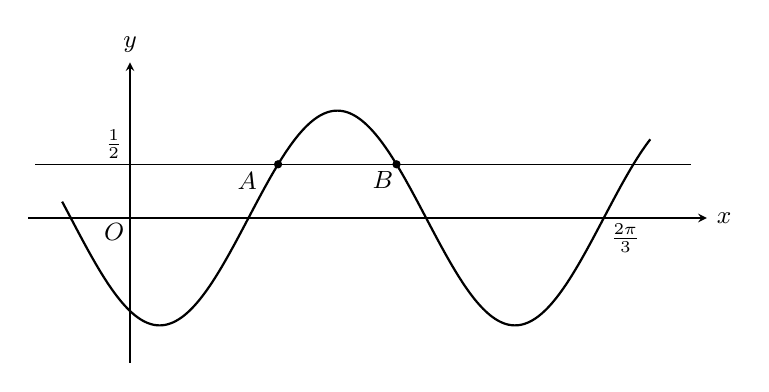
\begin{tikzpicture}
\begin{axis}[width=10.2cm, height=5.4cm, font=\small,
  axis lines=middle, xlabel={$x$}, ylabel={$y$},
  xmin=-0.45, xmax=2.55, ymin=-1.35, ymax=1.45,
  xtick=\empty, ytick=\empty,
  every axis x label/.style={at={(current axis.right of origin)}, anchor=west},
  every axis y label/.style={at={(current axis.above origin)}, anchor=south}]
  \addplot[domain=-0.42:2.48, samples=2] {0.5};
  \addplot[domain=-0.30:2.30, samples=300, thick] {sin(deg(4*x-2*pi/3))};
  \fill (axis cs:0.65450,0.5) circle (1.5pt);
  \fill (axis cs:1.17810,0.5) circle (1.5pt);
  \node[anchor=south east, inner sep=1pt] at (axis cs:-0.02,0.52) {$\frac{1}{2}$};
  \node[anchor=north east, inner sep=1pt] at (axis cs:0.575,0.455) {$A$};
  \node[anchor=north east, inner sep=1pt] at (axis cs:1.178,0.46) {$B$};
  \node[anchor=north west, inner sep=1pt] at (axis cs:2.11,-0.02) {$\frac{2\pi}{3}$};
  \node[anchor=north east, inner sep=1pt] at (axis cs:-0.01,-0.02) {$O$};
\end{axis}
\end{tikzpicture}
